\section{Authentifizierung}
\xxx[@rliebi: kapitel design = IST zustand. hier hat es vergleiche]
In diesem Kapitel werden verscheidene Methoden der Authentifizierung beleuchtet.
\subsection{Herkömmliche Registrierung per E-Mail}
Die herkömmliche Registrierung bietet den Vorteil, dass sie keine Abhängigkeiten zu Dritt-Providern erfordert. So kann sich jeder Benutzer mit einer gültigen E-Mail Adresse einloggen. Ein Nachteil dieser Methode kann sein, dass Dummy-Adressen verwendet werden können und so ein registrierter Benutzer nicht wirklich Authentifiziert ist.
\subsection{oAuth2}
oAuth2 hat einen anderen Ansatz. Sociale Netzwerke bieten sich an, um mit den Login-Daten des bereits bestehenden Accounts in einem solchen ein Account bei opendatahub zu erstellen. So ist der Benutzer der sich registriert bereits authentifizert und es kann davon ausgegangen werden, dass es sich wirklich um diesen handelt. Die häufigkeit von``Fake-Profilen'' wird dadurch reduziert.

\subsection{Cookie-Based-Authentication}
Bei der Cookie-Based-Authentifizierung wird eine Session-ID auf der Seite des Clients in einem Server-Side Cookie gespeichert. Dieses wird mit jedem Request an den Server übermittelt. So kann der Server davon ausgehen, dass es sich beim Client um den Inhaber der Session ID handelt.

\subsection{Token-Based-Authentication}
Ein neuerer Ansatz, ist es, einen Signierten Token im Header jedes Requests der zum Server geht mitzusenden. Vorteile dieser Variante sind bestechend:
\begin{description}
  \item[Cross-Domain / CORS]
  Cookies und CORS spielt nicht so sauber zwischen mehreren Domains. Ein Token basierter Ansatz erlaubt es AJAX Aufrufe an jeden Server mit jeder Domain zu veranlassen, weil die Informationen im HTTP Header liegen.
  \item[Stateless (Server-Side-Scalability)]Es wird kein Session-Store benötigt. Der Token enthält alle Benutzerinformationen der Rest des `States' liegt im Local Storage auf der Client-Side.
  \item[Decoupling] Man ist nicht an ein Authentifizierungs-Schema gebunden. Der Token kann überall generiert werden, sprich die API kann von überall her aufgerufen werden.
  \item[Mobile-Ready]Cookies sind in nativen mobilen Apps böse.
  \item[CSRF]Cross-Site Requests stellen kein Problem dar. Es gibt kein Authentication Cookie, das wiederverwendet werden könnte.
  \item[Standard]Es gibt bereits einen Standard. (\gls{JWT})
\end{description}
\begin{figure}[H]
    \centering
    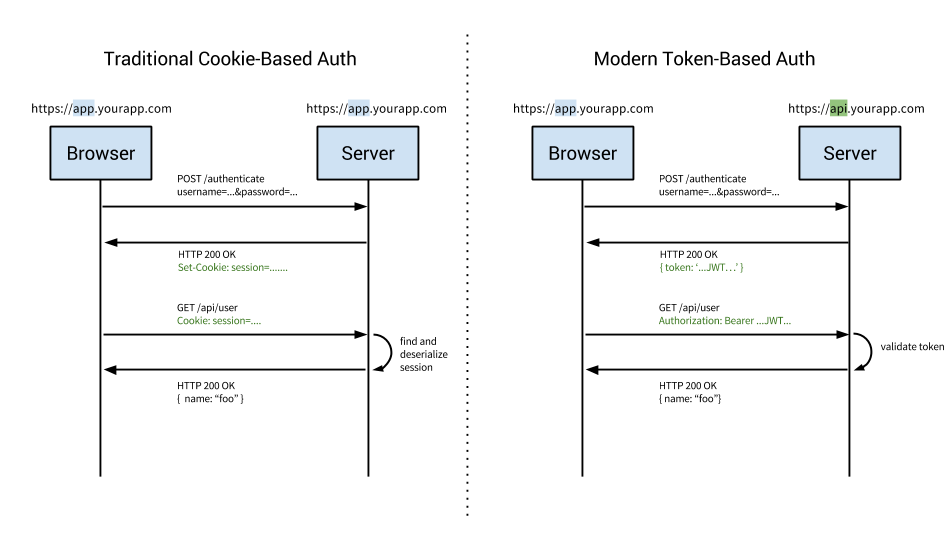
\includegraphics[width=\linewidth]{fig/cookie-token-auth}
    \caption{Vgl. Cookie vs. Token Auth}
    \label{fig:pd:cookie-token-auth}
\end{figure}